
\chapter{A new model for ${Ca^{2+}}$ signalling in fertilisation}

We have completed, in Chapter 2, a literature review of several $Ca^{2+}$ signalling models, focusing on the models by \citeA{atri} and by \citeA{lirinzel}. These are two minimal gating models that are still widely used. We have also studied in Chapter 3 the work by \citeA{Mak1998} which gives accurate data for the open probability of the $IP_3R$, $P_O$, as $[IP_3]$ and $[Ca^{2+}]$ vary. In this chapter we are going to present the derivation of a new model for $Ca^{2+}$ signalling in fertilisation. This will also be a gating model but, in an appropriate manner, it will incorporate for the first time the most up-to-date $IP_3R$ dynamics from \citeA{Mak1998}.

The \citeA{atri} model is a good starting point for creating a new gating model since it is a minimal model capturing many of the salient features of $Ca^{2+}$ signalling while not including an equation for $[Ca^{2+}]$ in the ER. Deciding how to best incorporate the equation for $P_O$ from \citeA{Mak1998} is not straightforward so we have explored several options. In the model by \citeA{swedish}, $P_O$ was inserted into the equation for cytosolic $Ca^{2+}$ as a multiplicative term for the flux entering the cytosol from the ER. This term is referred to as $J_{channel}$ in Chapter 4 (see equation \eqref{swedishvip3r}). We explored this idea but it does not quite fit in a gating model, {as gating models include terms for the $IP_3R$ dynamics in both ODEs, rather than just the equation for $Ca^{2+}$.} We, therefore, chose an alternative approach of splitting up the equation for $P_O$ given in \citeA{Mak1998} in an appropriate manner, as detailed below.

Revisiting the biological representation behind each term in the Atri model, \eqref{origatri1st}-\eqref{origatri2nd}, the probability of $IP_3$ binding to its activation site on the $IP_3R$ is represented by $p_1$, the probability of $Ca^{2+}$ binding to its activation site on the $IP_3R$ is represented by $p_2$, and the probability of $Ca^{2+}$ binding to the inhibitory site is represented by $p_3$. As given in Chapter 2, these probabilities are, respectively, given as follows:
\begin{align}
    p_1=\frac{p+\mu_0K_{IP_3}}{K_{IP_3}+p}, \qquad p_2=\frac{K_{act}b+c}{K_{act}+c}, \qquad p_3=\frac{K_{inh}^2}{K_{inh}^2+c^2}.\nonumber
\end{align}
To construct a new $Ca^{2+}$ signalling model, we split up the equation for $P_O$ in \citeA{Mak1998}, as follows:
\begin{align}
    P_{O1}&={\left(\frac{c^{H_{act}}}{c^{H_{act}}+K_{act}^{H_{act}}}\right)},\nonumber\\
    P_{O2}&={\left(\frac{K_{inh}^{H_{inh}}}{K_{inh}^{H_{inh}}+c^{H_{inh}}}\right),}\nonumber
\end{align}
where
\begin{equation}\nonumber
    K_{inh}=K_{\infty}\left(\frac{p^{H_{IP_3}}}{p^{H_{IP_3}}+K_{IP_3}^{H_{IP_3}}}\right).
\end{equation}
Here, $P_{O1}$ represents the probability of $Ca^{2+}$ binding to the activation site on the $IP_3R$ and depends on the half-maximal activation constant, $K_{act}$, and on the Hill coefficient, $H_{act}=1.9 \pm 0.3$. $P_{O1}$ increases with $Ca^{2+}$. $P_{O2}$ represents the probability of $Ca^{2+}$ binding to its inhibitory site. This depends on $Ca^{2+}$ and $K_{inh}$, where $K_{inh}$ depends on $IP_3$. As $[Ca^{2+}]$ increases, $P_{O2}$ decreases. As $[IP_3]$ increases, $K_{inh}$ increases, and hence $P_{O2}$ increases. Plots of $P_{O1}$ as a function of $Ca^{2+}$ and $P_{O2}$ as a function of $Ca^{2+}$ and $IP_3$ can be seen in Figures \ref{parenthcomparison}\textbf{A} and \ref{parenthcomparison}\textbf{C}.

To construct a new $Ca^{2+}$ signalling model from the Atri model, we replace $p_1p_2$ in $J_{channel}$ (in equation \eqref{origatri1st} for cytosolic $Ca^{2+}$) with $P_{O1}$. Moreover, we replace $p_3$ (in equation \eqref{origatri2nd} for the proportion of non inactivated $IP_3R$) with $P_{O2}$. Plotting $p_1$, $p_2$, $p_3$, $P_{O1}$, $P_{O2}$ as functions of $Ca^{2+}$ and $IP_3$ in Figure \ref{parenthcomparison}, we observe similarities and differences. In Figures \ref{parenthcomparison}\textbf{A} and \ref{parenthcomparison}\textbf{B}, we see that $P_{O1}$ behaves similarly to $p_1p_2$. Note that the scales are slightly different here as $k_{flux}$ is a multiplicative factor in the $J_{channel}$ term in the Atri model. However, in Figures \ref{parenthcomparison}\textbf{C} and \ref{parenthcomparison}\textbf{D}, we see that $P_{O2}$ and $p_3$ behave very differently. As the $IP_3$ concentration increases, $p_3$ does not change very much. In contrast, there is a far more significant change in $P_{O2}$ as $[IP_3]$ increases, particularly for lower levels of $IP_3$. This $IP_3R$ behaviour emerging from the experiments in \citeA{Mak1998} is a crucial feature included in our new model. Figure \ref{parenthcomparison}\textbf{F} shows $p_1p_2p_3$ vs. $IP_3$ for different levels of $Ca^{2+}$. For lower levels of $Ca^{2+}$, $p_1p_2p_3$ barely changes as $[IP_3]$ changes. The dependence on higher levels of $Ca^{2+}$ is also very minimal. In comparison, there is clearly far more change in $P_{O1}P_{O2}$ as $[Ca^{2+}]$ and $[IP_3]$ vary, as seen in Figure \ref{parenthcomparison}\textbf{E}. Similarly, in Figure \ref{fig3datrifoskett}\textbf{A} we plot $p_1p_2p_3$ vs. $IP_3$ for selected levels of $Ca^{2+}$ and this can be compared to Figure \ref{fig3datrifoskett}\textbf{B} where we plot $P_O$ vs. $Ca^{2+}$ and $IP_3$. We see once again that $p_1p_2p_3$ from the Atri model does not change significantly with increasing levels of $IP_3$, whereas $P_{O1}P_{O2}$ from \citeA{Mak1998} does.

\begin{figure}[h!!!t!!!b!!!p]
  \centering
  \includegraphics[width=1\linewidth]{Chapters/5_New_Model/extras/PARENTHCOMPARISONnew.png}
  \caption{(\textbf{A}) $P_{O1}$ vs. $[Ca^{2+}]$ and $[IP_3]$. (\textbf{B}) $p_1p_2$ vs. $[Ca^{2+}]$ and $[IP_3]$. (\textbf{C}) $P_{O2}$ vs. $[Ca^{2+}]$ and $[IP_3]$. (\textbf{D}) $p_3$ vs. $[Ca^{2+}]$ and $[IP_3]$. (\textbf{E}) $P_{O}=P_{O1}P_{O2}$ vs. $Ca^{2+}$ and $IP_3$. (\textbf{F}) $p_1p_2p_3$ vs. $Ca^{2+}$ and $IP_3$. $P_{O1}$ and $P_{O2}$ are from \citeA{Mak1998}. $p_1$, $p_2$ and $p_3$ are from \citeA{atri}. \textit{Software:} MATLAB. }\label{parenthcomparison}
\end{figure}

\begin{figure}[h!!!t!!!b!!!p]
\centering
  \minipage{0.8\textwidth}
  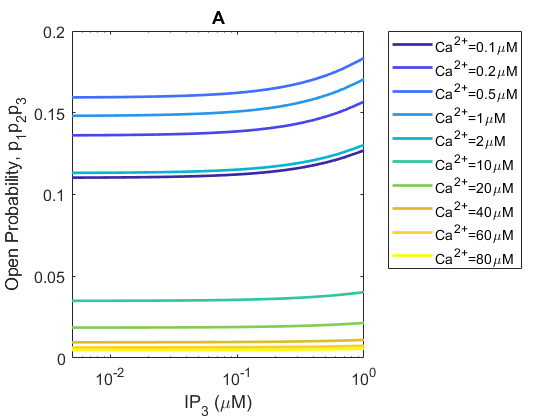
\includegraphics[width=\linewidth]{Chapters/5_New_Model/extras/fig3cfoskettmatlabATRI.png}
\endminipage\hfill
\minipage{0.8\textwidth}
  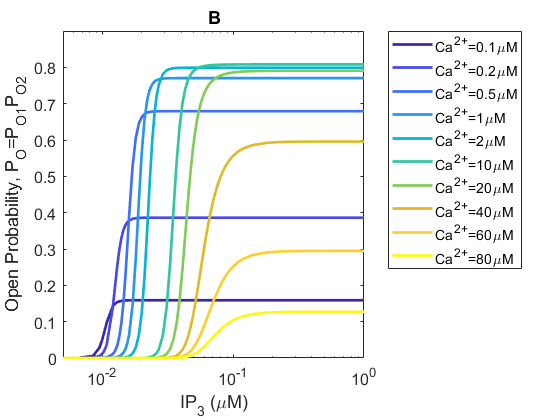
\includegraphics[width=\linewidth]{Chapters/5_New_Model/extras/anotherfoskettfig3c.png}
\endminipage\hfill
  \caption{(\textbf{A}) $p_1p_2p_3$ (Atri model) vs. cytosolic $IP_3$ concentrations at various levels of cytosolic $[Ca^{2+}]$. Parameter values used are shown in Table \ref{origatriparam}. (\textbf{B}) $P_{O1}P_{O2}$ (Mak et al., 1998) vs. cytosolic $IP_3$ concentrations at various levels of cytosolic $[Ca^{2+}]$. Parameter values used are shown in Table \ref{foskettparam}. {The $Ca^{2+}$ values here were chosen to mirror the ones used in figure 3c in \shortciteA{Mak1998}.} \textit{Software:} MATLAB. }\label{fig3datrifoskett}
\end{figure}

Finally, Figures \ref{fosketthillfunctionatri}\textbf{A} and \ref{fosketthillfunctionatri}\textbf{B} are compared. In the former, $p_1p_2p_3$ is plotted as $[Ca^{2+}]$ increases for different levels of $[IP_3]$. We see that $p_1p_2p_3$ does not change as $[IP_3]$ goes from $0.01\mu M$ to $0.1\mu M$. It does change significantly when $[IP_3]$ reaches $10 \mu M$ though. This once again illustrates that in the Atri model, the open probability of the $IP_3R$ does not vary much at low levels of $[IP_3]$. In contrast, the $IP_3R$ dynamics derived in \citeA{Mak1998} depend on $[IP_3]$ and $[Ca^{2+}]$ significantly, as seen in Figure \ref{fosketthillfunctionatri}\textbf{B}. These comparisons demonstrate the importance of implementing the $IP_3R$ dynamics from \citeA{Mak1998} in a new model.


\begin{figure}[h!!!t!!!b!!!p]
  \centering
  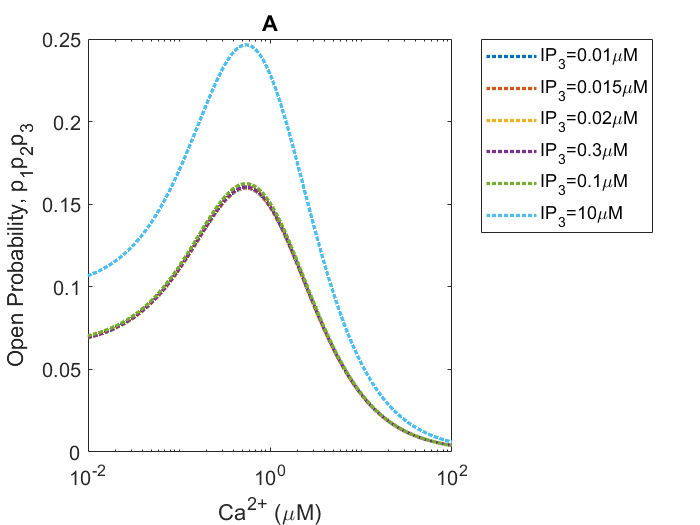
\includegraphics[width=0.8\linewidth]{Chapters/5_New_Model/extras/fosketthillfunctionATRI.png}
  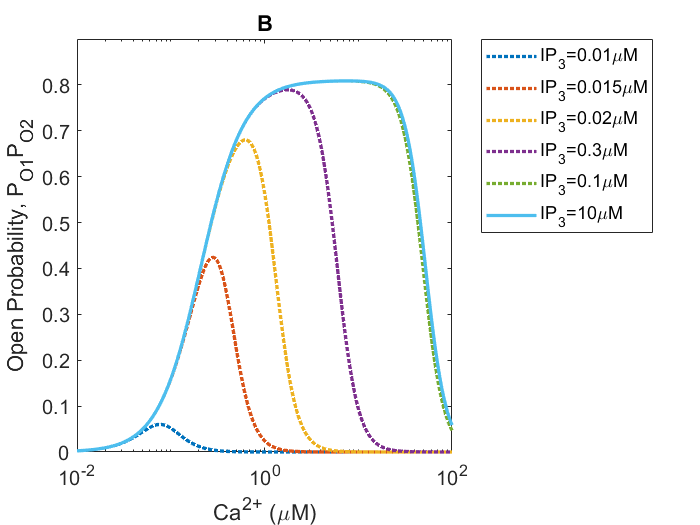
\includegraphics[width=0.8\linewidth]{Chapters/5_New_Model/extras/anotherfosketthill.png}
  \caption{(\textbf{A}) $p_1p_2p_3$ (from the Atri model) as a function of cytosolic $Ca^{2+}$ for various $IP_3$ levels of interest. Parameter values used are shown in Table \ref{origatriparam}. (\textbf{B}) $P_{O1}P_{O2}$ (from Mak et al., 1998) as a function of cytosolic $Ca^{2+}$ for various $IP_3$ levels of interest. Parameter values used are shown in Table \ref{foskettparam}. \textit{Software:} MATLAB.}\label{fosketthillfunctionatri}
\end{figure}

One less researched $Ca^{2+}$ flux is that of the SERCA pump, modelled by $J_{pump}$ in equation \eqref{origatri1st}. \citeA{atri} used a simple Hill function to model it and acknowledged it could be improved when more experimental data would be made available. For this reason we use more recent $Ca^{2+}$ models to improve this term. In particular, we use the expression {$V_ec^2/(K_e^2+c^2)$} from \citeA{hofer} who derived a sophisticated gating model with cytosolic $Ca^{2+}$, the proportion of non inactivated $IP_3R$, $Ca^{2+}$ in the ER and $IP_3$ as dynamic variables. They used a SERCA pump flux term with a Hill coefficient of 2, and the half-activation constant was given as $K_e=0.1 \mu Ms^{-1}$. These parameter values are based on \shortciteA{lyttonetal} and \shortciteA{carmelloetal}.

Summarising, the inclusion of the $IP_3R$ dynamics from \citeA{Mak1998} and the SERCA pump flux term from \citeA{hofer} leads us to a new model for $Ca^{2+}$ signalling in fertilisation:
\begin{align}
    \frac{dc}{dt}=&K_{flux}nP_{O1}-\frac{V_ec^2}{K_e^2+c^2},\label{newnew1}\\
    \frac{dn}{dt}=&g(P_{O2}-n).\label{newnew2}
\end{align}
{This model has qualitative agreement to the data \shortcite{Mak1998}.} Note that mouse eggs oscillate for some time in a $Ca^{2+}$-free medium \cite{Sanders2018}. One can `isolate' mouse eggs so that no efflux or influx takes place and in this case, they can oscillate for many hours \cite{wakai}. This implies that $Ca^{2+}$ exchange with the extracellular medium is not necessary for $Ca^{2+}$ oscillations (page 246 in \citeA{dupont}), \cite{YaoParker1994}. Hence, in the Atri model, the $J_{leakage}$ term is not essential for $Ca^{2+}$ oscillations. We therefore disregard any leakage flux component in our model.

The next step is to perform a linear stability analysis of the model \eqref{newnew1}-\eqref{newnew2} and show that the model can generate oscillations for a range of $IP_3$ values that are compatible with experimental findings.

\section{Linear stability analysis}
We will now carry out the linear stability analysis of our new model \eqref{newnew1}-\eqref{newnew2} in order to determine if an oscillatory regime exists and for which $IP_3$ values. In \citeA{Mak1998} a range for each parameter value is given. We use values in these ranges, and we also use the half-activation constant in $J_{pump}$ as in the \citeA{hofer} model. We leave $k_{flux}$ and $V_e$ undetermined mutually. We know that $k_{flux}$ measures the maximum flux from the ER to the cytosol, and $V_e$ measures the maximum flux from the cytosol to ER. We assume that proteins are constant in a cell over the period of oscillations. We can also expect steady states of around $0.1 \mu M$ for $Ca^{2+}$ \cite{Berridge, kline}, and $n$ varies between $0$ and $1$ since it represents a proportion. Additionally, we must ensure a steady state value of approximately $0.01 \mu M$ for $IP_3$ \cite{Mak1998,karl}. This is a reasonable assumption since it is below the level that stimulates the opening of the $IP_3R$.

We set $dc/dt=dn/dt=0$ to find the steady states. We have
\begin{align}
    F(c,n)=&k_{flux}n{\left(\frac{c^{H_{act}}}{c^{H_{act}}+K_{act}^{H_{act}}}\right)}-\frac{V_ec^2}{K_e^2+c^2}\nonumber\\
    =&0,\label{newnewnew1}\\
    G(c,n)=&g{\left(\frac{K_{inh}^{H_{inh}}}{K_{inh}^{H_{inh}}+c^{H_{inh}}}-n\right)}\nonumber\\
    =&0,\label{newnewnew2}
\end{align}
where
\begin{equation}
    K_{inh}=K_{\infty}\frac{p^h_{IP_3}}{p^{h_{IP_3}}+k_{IP_3}^{h_{IP_3}}},\nonumber
\end{equation}
where we have four unknowns: $c$, $n$, $k_{flux}$, and $V_e$.

We then determine the Trace, Determinant, and Discriminant of the Jacobian matrix of the system \eqref{newnewnew1} and \eqref{newnewnew2}. The partial derivatives are
\begin{align}
    \frac{\partial F}{\partial c}=&\frac{k_{flux}nc^{H_{act}}H_{act}}{c(c^{H_{act}}+{K_{act}}^{H_{act}})}-\frac{k_{flux}n(c^{H_{act}})^2{H_{act}}}{(c^{H_{act}}+{K_{act}}^{H_{act}})^2c}-\frac{2V_ec}{{K_e}^2+c^2}+\frac{2{V_e}c^3}{({K_e}^2+c^2)^2},\\
    \frac{\partial F}{\partial n}=&\frac{k_{flux}c^{H_{act}}}{c^{H_{act}}+{K_{act}}^{H_{act}}},\\
    \frac{\partial G}{\partial c}=&-g\frac{\left(\frac{K_{\infty}p^{h_{IP_3}}}{{p^{h_{IP_3}}+{k_{IP_3}}}^{h_{IP_3}}}\right)^{H_{inh}}c^{H_{inh}}H_{inh}}{\left(\left(\frac{K_{\infty}p^{h_{IP_3}}}{p^{h_{IP_3}}+{k_{IP_3}}^{h_{IP_3}}}\right)^{H_{inh}}+c^{H_{inh}}\right)^2c},\\
    \frac{\partial G}{\partial n}=&-g.
\end{align}
Hence, the Trace, Determinant and Discriminant are defined respectively as follows:
\begin{align}
    &T(c,n)=\frac{\partial F}{\partial c}+\frac{\partial G}{\partial n},\nonumber\\
    &D(c,n)=\frac{\partial F}{\partial c}\frac{\partial G}{\partial n}-\frac{\partial F}{\partial n}\frac{\partial G}{\partial c},\nonumber\\
    &Disc(c,n)=(T(c,n))^2-4D(c,n).\nonumber
\end{align}
Solving equations \eqref{newnewnew1} and \eqref{newnewnew2} and setting constraints so that $T(c,n)>0$, $D(c,n)>0$, $Disc(c,n)<0$, we obtain appropriate steady state values and parameters values for $k_{flux}$ and $V_e$. The steady states obtained are $c_s = 0.08 \mu M$ and $n_s = 0.60$ (which are within a reasonable range \cite{Berridge,kline,karl}) when $k_{flux}=4.89$, $V_e=1$.

\begin{figure}[h!!!t!!!b!!!p]
  \centering
  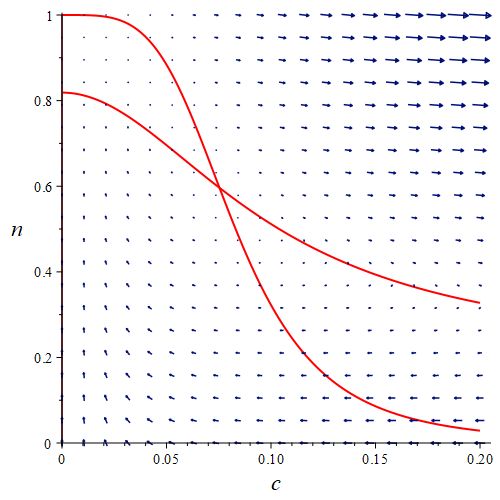
\includegraphics[width=0.6\linewidth]{Chapters/5_New_Model/extras/A_vectorfield.png}
  \caption{The nullclines of the system \eqref{newnewnew1}-\eqref{newnewnew2}, with $k_{flux}=4.89$, $V_e=1$ and parameter values as given in Table \ref{tablewithhofersquared}. The steady state is where the lines intersect. {Arrows indicate the vector field.} \textit{Software:} Maplesoft.}
\end{figure}

Evaluating the Trace, Determinant and Discriminant at the steady state value $c=0.08$ gives:
\begin{align}
T(c_s,n_s)&= 1.79,\nonumber\\
D(c_s,n_s)&=2.74,\nonumber\\
Disc(c_s,n_s)&= -7.76.\nonumber
\end{align}

\section{Simulations}
We have completed the linear stability analysis, and decided on parameter values shown in Table \ref{tablewithhofersquared}.

\begin{figure}[h!!!t!!!b!!!p]
  \centering
  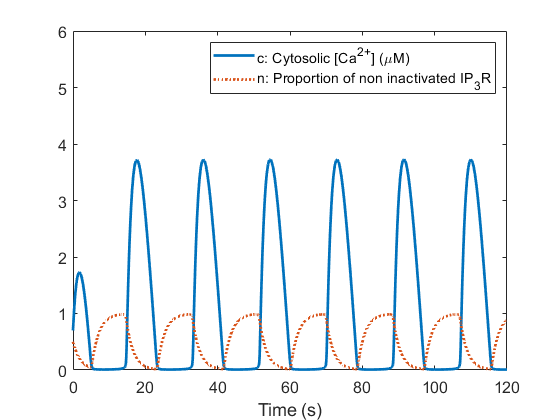
\includegraphics[width=0.8\linewidth]{Chapters/5_New_Model/extras/hofersquared.png}
  \caption{$Ca^{2+}$ oscillations arising from the system \eqref{newnew1}-\eqref{newnew2}, blue solid lines, with $p=0.01 \mu M$. The proportion of non inactivated $IP_3R$ is also plotted, with a red dashed line. Parameter values are given in Table \ref{tablewithhofersquared}. \textit{Software:} MATLAB.}\label{hofersquared}
\end{figure}

Oscillations generated by the model \eqref{newnew1}-\eqref{newnew2} can be seen in Figure \ref{hofersquared}, where $p=0.01 \mu M$. Our model reproduces
the low frequency, large amplitude oscillations characteristic of fertilising mammalian eggs (shown in Figure \ref{karlfig2}). We need to examine the exact range of values of $p$ for which these oscillations exist, if the oscillations change in that range, and if the experimental findings in \citeA{Sanders2018} are replicated. 

We can determine the range of $p$ for which the ODE system \eqref{newnew1}-\eqref{newnew2} yields oscillations by plotting the Trace, Determinant, and Discriminant at the steady states, and determining the range for which $T>0$, $D>0$, and $Disc<0$ (unstable spiral). We find that this range is $0.0085 \leq p \leq 0.014$ which is extremely small. This can be seen in Figure \ref{tdd}. 

\begin{figure}[!htb]
\centering
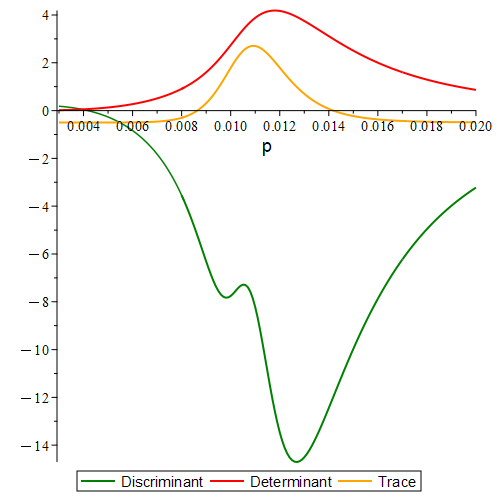
\includegraphics[width=0.7\linewidth]{Chapters/5_New_Model/extras/mapletdd.png}
\caption{{Trace, Determinant, and Discriminant for the system of equations \eqref{newnewnew1}-\eqref{newnewnew2} for varying bifurcation parameter $p$. Parameter values are as in Table \ref{tablewithhofersquared}.} \textit{Software:} MATLAB.}\label{tdd}
\end{figure}

In order to enlarge the range of $p$ to be $0.01 \mu M \leq [IP_3] \leq 1 \mu M$ for which the system is oscillatory, a non-linear scaling of equation \eqref{newnew1} would be needed. Unfortunately, this is beyond the scope of this project.  This scaling should render the left Hopf point at approximately $[IP_3]=0.01 \mu M$, and the right Hopf point at $[IP_3] \approx 1 \mu M$ \cite{karl}.

Regardless of the oscillatory range of $p$ being an order of magnitude inaccurate, we can still analyse the behaviour of the oscillations. Figure \ref{tdd} shows the oscillations for $p=0.0085$ and $p=0.014$, respectively, at each end of the oscillatory range. Both the amplitude and frequency of oscillations increase as the $IP_3$ concentration is increased, as seen in experiments \cite{Sanders2018}. However, the amplitude increase is more pronounced that the frequency increase.

\begin{figure}[!htb]
\centering
\minipage{0.8\textwidth}
  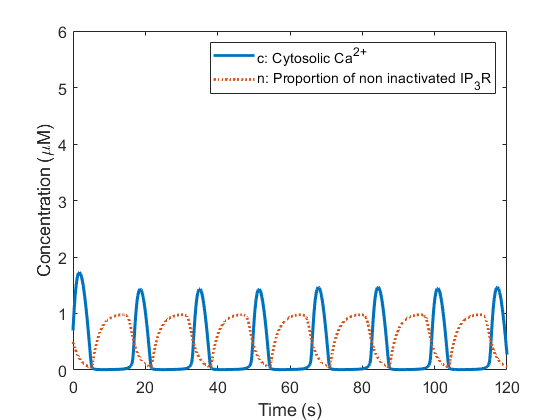
\includegraphics[width=\linewidth]{Chapters/5_New_Model/extras/p00085.png}
\endminipage\hfill\\
\minipage{0.8\textwidth}
  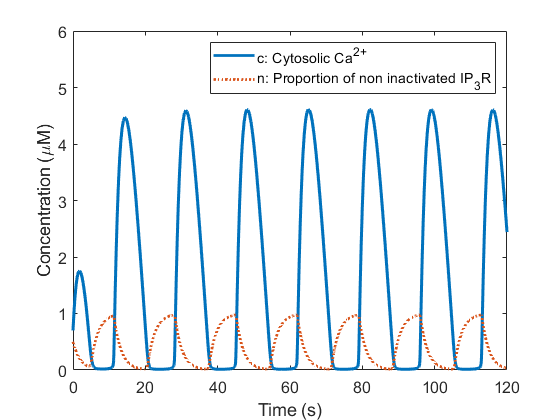
\includegraphics[width=\linewidth]{Chapters/5_New_Model/extras/p0014.png}
\endminipage\hfill
\caption{$Ca^{2+}$ oscillations exhibited by new model \eqref{newnew1}-\eqref{newnew2}, for \textbf{(a)} $p=0.0085$ and \textbf{(b)} $p=0.014$. We observe both ends of oscillatory region. \textit{Software:} MATLAB.}\label{tdd}
\end{figure}

Our new model \eqref{newnew1}-\eqref{newnew2} produces $Ca^{2+}$ oscillations of higher frequency when there is a higher concentration of $IP_3$ present in the cytosol. This result is in agreement with the experiments by \citeA{Sanders2018}. Previous models of $Ca^{2+}$ signalling  \cite{atri,lirinzel,deyoungkeizer,Sanders2018,Theodoridou2013} have assumed outdated $IP_3R$ dynamics, and instead relied on the ER store refilling to drive oscillations. We know that this is not the case for $Ca^{2+}$ signalling in fertilisation \cite{Sanders2018, wakai}. We have managed to reproduce key aspects of the experimental findings of \citeA{Sanders2018} with our new two--variable model which incorporates the correct $IP_3R$ dynamics from \citeA{Mak1998}. However, the data from \citeA{Sanders2018} and \citeA{sneyd} show that $IP_3$ concentration is not constant and needs to be a dynamic variable in a $Ca^{2+}$ model for fertilising eggs. Obtaining a new model closer to the data from \citeA{Sanders2018} and \citeA{Mak1998} was of foremost importance and is the first step to reaching a more complex three--variable model with dynamic $IP_3$. {We have derived a model that does not depend on the ER store emptying and refilling, as the data from \shortciteA{Sanders2018} and \shortciteA{wakai} suggest. We have also managed to incorporate the $IP_3R$ dynamics for fertilisation, that accurately depend on $[Ca^{2+}]$ and $[IP_3]$, as found by \shortciteA{Mak1998}.} The next step of incorporating an ODE for $IP_3$ is beyond the scope of this project and is left for future work.

Note that the data from \citeA{sneyd} are in agreement with the data from \citeA{Sanders2018}, though experiments were carried out on pancreatic acinar cells and airway smooth muscle cells. \citeA{sneyd} also derived two models with an ODE for $IP_3$, based on the Atri model and the Li-Rinzel model. We study these models in Appendix A.

\begin{table}[h!!!t!!!b!!!p]
\begin{center}
\begin{tabular}{ c c }
Parameters used in new model & Value\\
\hline
$K_{flux}$ & $8.6$ {$\mu M s^{-1}$}\\
\hline
$K_{act}$ & $0.2$ {$\mu M$}\\
\hline
$H_{act}$ & $2$\\
\hline
$V_e$ & $1$ {$\mu M s^{-1}$}\\
\hline
$K_e$ & $0.1$ {$\mu M$}\\
\hline
$K_{\infty}$ & $52$ {$\mu M$}\\
\hline
$K_{IP_3}$ & $0.05$ {$\mu M$}\\
\hline
$H_{IP3}$ & $4$\\
\hline
$g$ & $0.5$\\
\hline
$h$ & $0.5$
\end{tabular}
\end{center}
\caption{Parameters used in new model, \eqref{newnew1}-\eqref{newnew2}. }\label{tablewithhofersquared}
\end{table}